
\frame{
\frametitle{Signaalityypit ja signaalinkäsittely}
\begin{block}{Määritelmä}
\begin{itemize}
\item Signaali = tietoa välittävä merkki.\footnote{Kielitoimiston sanakirja 2.0}
\item Signaali = ajan tai paikan mukaan muuttuva mitattava suure, jonka muutoksia voidaan käsitellä datana.\footnote{Tietotekniikan liiton ATK-sanakirja 5.0}
\end{itemize}
\end{block}
\begin{block}{Määritelmä}
Signaalinkäsittely = lukujonon muotoon saatetun signaalin käsittely, yleensä tietokoneella, signaalin kantaman informaation esille saamikseksi
Signaalinkäsittelyn menetelmiä ovat mm. signaalin suodattaminen, erottelu muista signaaleista, virheiden korjaaminen tai havainnollisuuden parantaminen. Yleisimmin käsitellään kuva-, ääni-, puhelin-, radio- ja mittaussignaaleja.\footnote{Tietotekniikan liiton ATK-sanakirja 5.0}
\end{block}
}


\frame{
\begin{center}
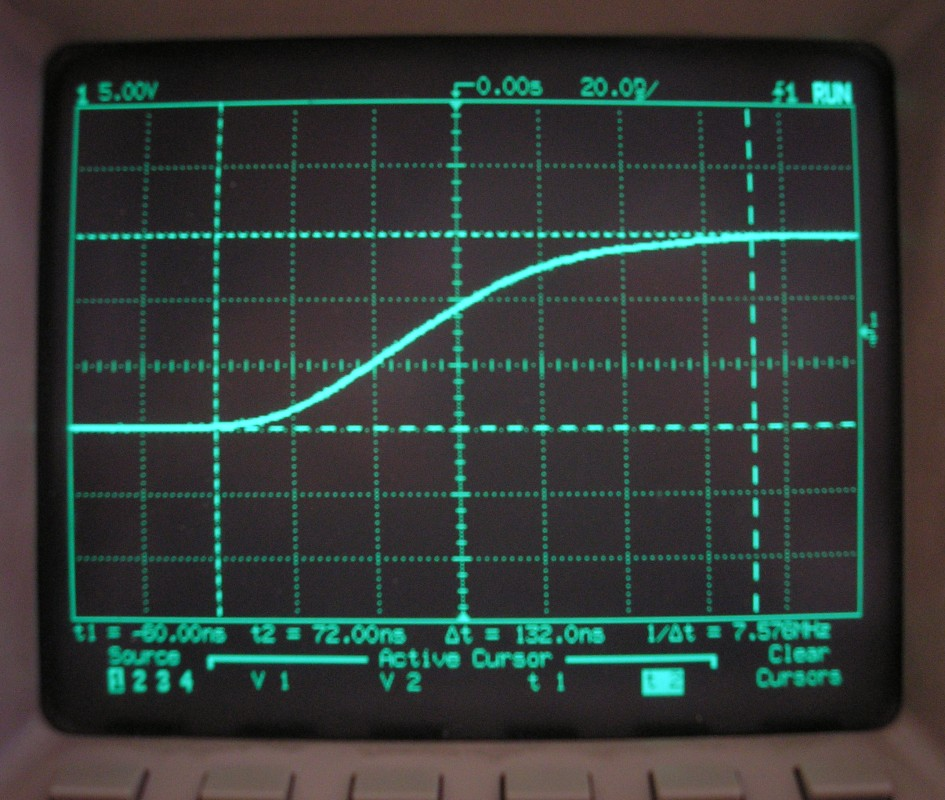
\includegraphics[height=8.4cm]{signaalit_pics/Digital_oscilloscope.jpg}\\
\tiny \url{http://commons.wikimedia.org/wiki/File:Digital\_oscilloscope.jpg}
\end{center}
}

\frame{
\begin{center}
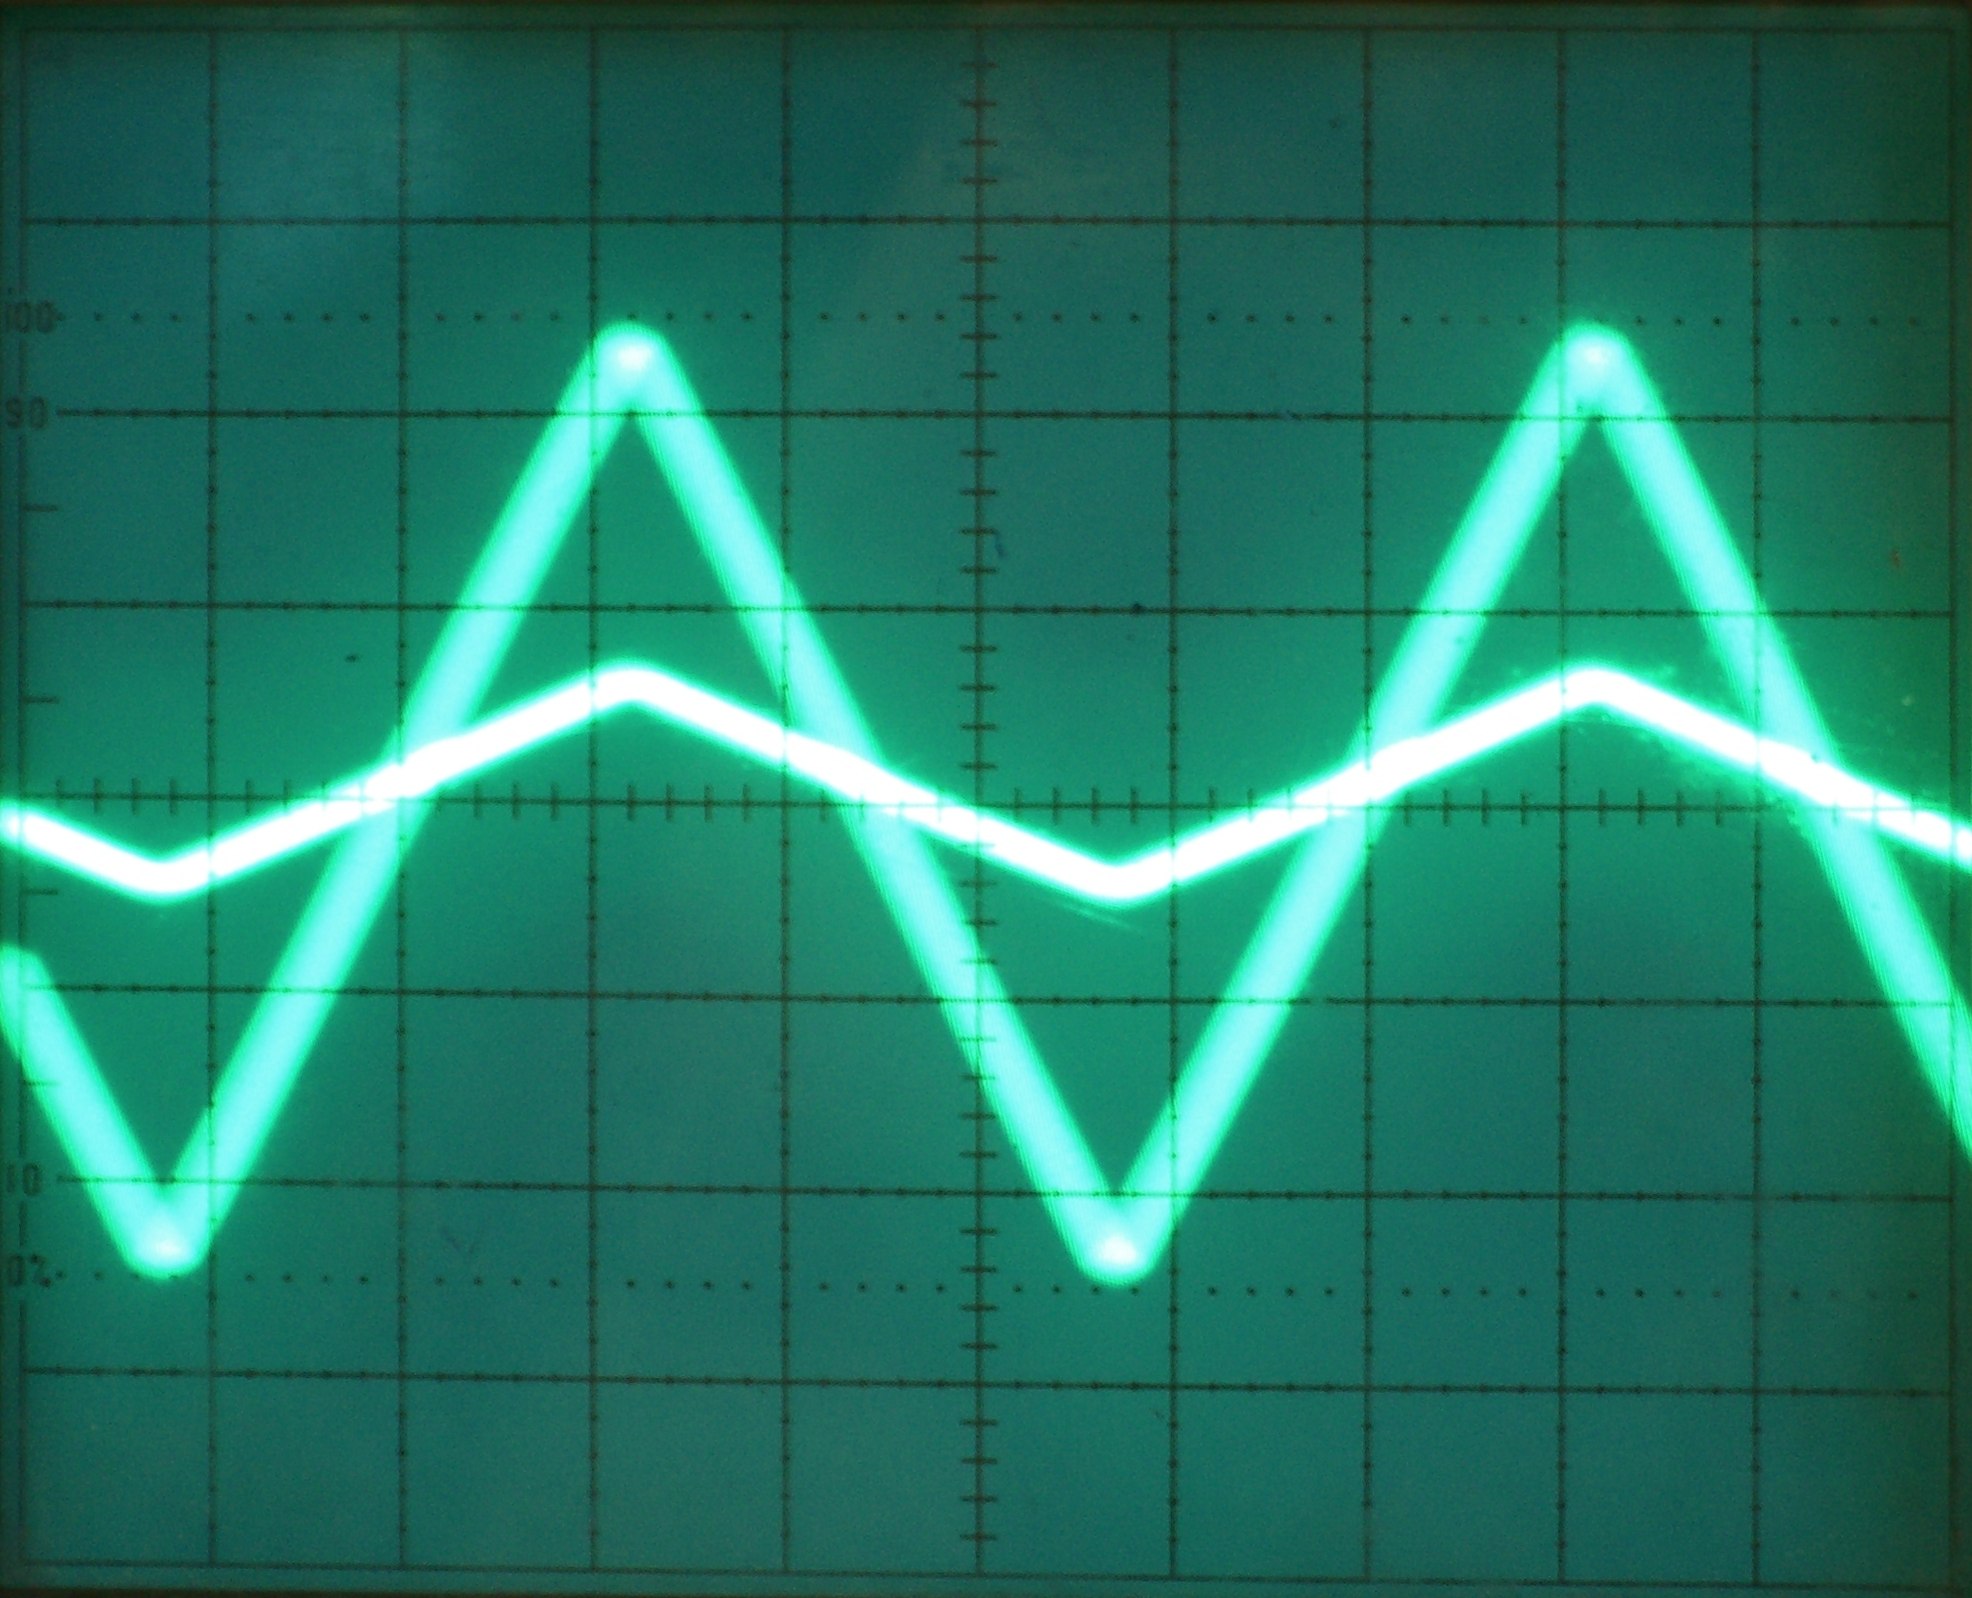
\includegraphics[height=8.4cm]{signaalit_pics/Oscilloscope_Triangle_Wave.jpg}\\
\tiny \url{http://commons.wikimedia.org/wiki/File:Oscilloscope\_Triangle\_Wave.jpg}
\end{center}
}

\frame{
\begin{center}
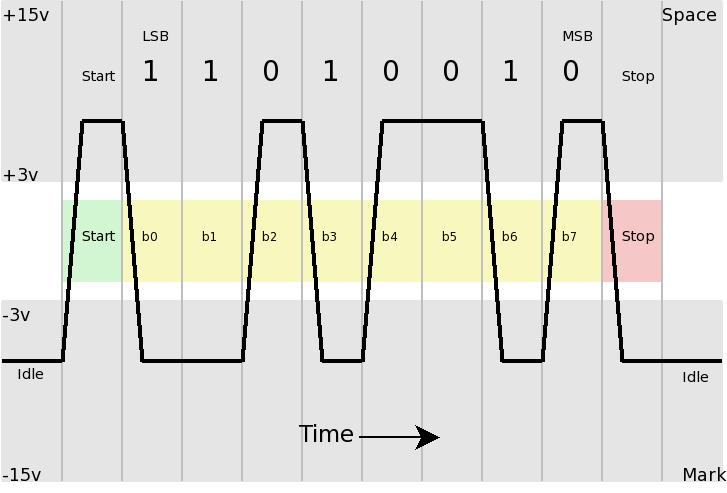
\includegraphics[height=8.1cm]{signaalit_pics/Rs232_oscilloscope_trace.jpg}\\
\tiny \url{http://commons.wikimedia.org/wiki/File:Rs232\_oscilloscope\_trace.jpg}
\end{center}
}

\frame{
\frametitle{Fourier'n teoreema}
Mikä tahansa jaksollinen signaali voidaan hajottaa siniaaltojen summaksi, valitsemalla
siniaalloille sopivat amplitudit, taajuudet ja vaihe-erot. Tätä summaa kutsutaan Fourier-sarjaksi.
Sähköisen signaalin Fourier-sarja muodostuu tasajännitekomponentista, perustaajuudesta ja perustaajuuden
monikerroista.

Hyvä esimerkki:\\
\url{http://commons.wikimedia.org/wiki/File:Fourier\_synthesis\_square\_wave\_animated.gif}

}


\frame{
\begin{center}
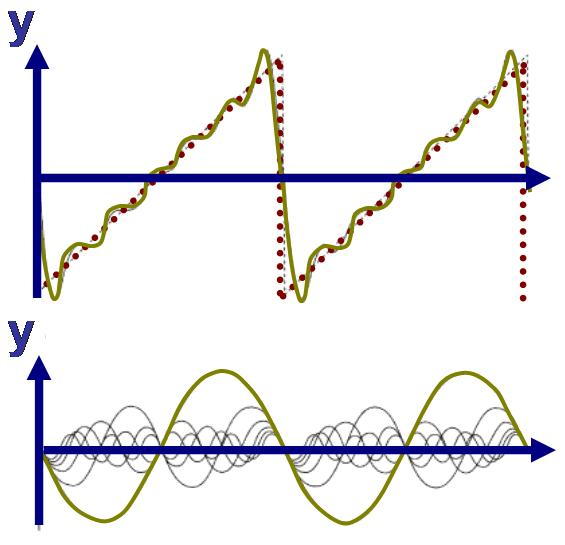
\includegraphics[height=8.4cm]{signaalit_pics/Sawtooth_Fourier_Analysis.JPG}\\
\tiny \url{http://commons.wikimedia.org/wiki/File:Sawtooth\_Fourier\_Analysis.JPG}
\end{center}
}

\frame{
\frametitle{Digitaalinen vs. analoginen}
\begin{itemize}
\item Analoginen signaali: signaali voi saada mitä tahansa arvoja, ja muuttua miten tahansa
ajan funktiona.
\item Digitaalinen signaali: signaalilla on määrätyt vakioarvot, ja se muuttuu ennalta sovitulla
tavalla (esim. 1000 000 kertaa sekunnissa).
\item Yleisesti käytössä oleva digitaalitekniikka käyttää binäärilogiikkaa, eli signaalilla on
kaksi sallittua tilaa, 0 ja 1.
\end{itemize}
}

\frame{
\frametitle{Digitaalinen vs. analoginen} % http://en.wikipedia.org/wiki/Analog_recording_vs._digital_recording
\begin{itemize}
\item Kun vertaat digitaalisia ja analogisia järjestelmiä, mitä eroja sinulle tulee mieleen?
\item Vinyyli vs. cd-levy? Analoginen televisio vs. digitelevisio?
\end{itemize}
}


\frame{
\frametitle{Signaalityypit}
Signaalit voidaan jakaa karkeasti analogisiin ja digitaalisiin signaaleihin. Tarkempi jako voidaan suorittaa jatkuva- ja diskreettiamplitudisiin sekä jatkuva- ja diskreettiaikaisiin signaaleihin. Esimerkkejä:
\begin{itemize}
\item Audiosignaali (vaikkapa mikrofonin tai kaiuttimen kaapelista mitattuna) on sekä jatkuva-aikainen että jatkuva-amplitudinen.

\item Ikkunannostimen rajakytkimeltä saatava signaali on diskreettiamplitudinen: sillä on kaksi tilaa, auki ja kiinni. Sen sijaan signaali on jatkuva-aikainen.

\item CD-levylle tallennettu musiikki on signaalina sekä diskreettiamplitudinen että diskreettiaikainen. Se on muodostettu audiosignaalista kvantisoimalla ja näytteistämällä.

\item Diskreettiaikaisesta mutta jatkuvasta signaalista on hankalampi keksiä jokapäiväistä esimerkkiä.
\end{itemize}
}



\frame{
\frametitle{Kvantisointi ja näytteistys}
\begin{block}{Kvantisointi}
Jatkuva-amplitudinen signaali muutetaan diskreettiamplitudiseksi kvantisoimalla. Mitä tarkemmin signaali halutaan tallentaa, sitä enemmän näytteistystasoja tarvitaan. Esimerkiksi cd-levyllä yksi ääninäyte tallennetaan 16 bitillä, eli mahdollisia tasoja on $2^{16}=65 536$.
\end{block}
\begin{block}{Näytteistys}
Jatkuva-aikainen signaali muutetaan diskreettiaikaiseksi näytteistämällä. Mitä suurempi taajuusalue halutaan tallentaa, sitä suurempi pitää näytteenottotaajuuden olla. Esimerkiksi cd-levyllä näytteenottotaajuus on 44,1 kHz, eli äänisignaalista tallennetaan näyte 44100 kertaa sekunnissa.
\end{block}
}

\frame{
\frametitle{Nyquistin näytteenottoteoreema}
Nyquistin näytteenottoteoreeman mukaan näytteenottotaajuuden on oltava vähintään kaksinkertainen verrattuna suurimpaan signaalitaajuuteen.

Esimerkiksi jos haluamme tallentaa ääntä taajuusalueella 0 Hz -- 20\,000 Hz, näytteenottotaajuuden on oltava
vähintään 40\,000 kHz.
}

\frame{
\frametitle{Laskostuminen}
Jos näytteenottotaajuus on $f_{\rm s}$, niin voimme tallentaa signaalit aina taajuuteen $f_{\rm s}/2$ asti. Taajuudet, jotka ovat suurempia kuin $f_{\rm s}/2$, on
suodatettava pois ennen näytteistystä, muuten ne siirtyvät haittasignaaliksi varsinaiselle taajuusalueelle eli {\em laskostuvat}. Esimerkiksi taajuudella $2f_{\rm s}+10\ Hz$ esiintyvä haittasignaali siirtyy hyötykaistalle taajuudelle 10 Hz.
\begin{center}
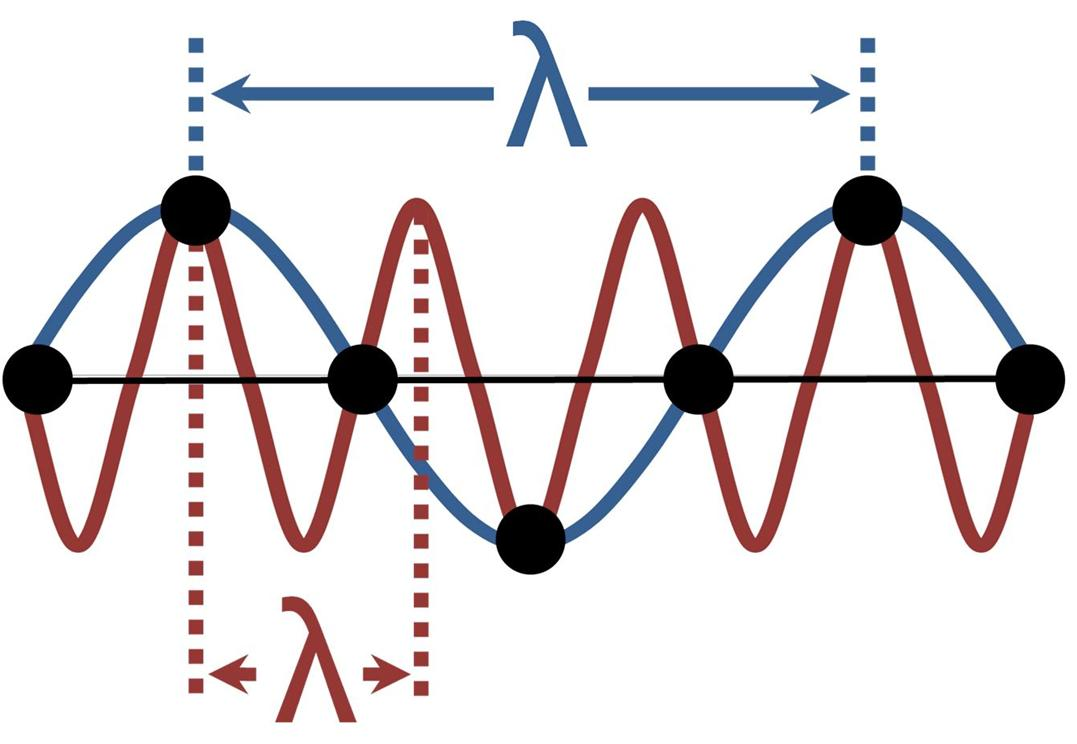
\includegraphics[height=4cm]{signaalit_pics/Wavelength_indeterminacy.JPG}\\
\tiny \url{http://commons.wikimedia.org/wiki/File:Wavelength\_indeterminacy.JPG}
\end{center}
}




\frame{
\frametitle{Kohina}
Kohina = hyötysignaalia häiritsevä satunnaisesti vaihteleva häiriö. Sähkölaitteissa kohinan lähteitä ovat
muun muassa
\begin{description}
\item[Taustakohina] Avaruudesta säteilynä välittyvä taustakohina.
\item[Lämpökohina] Varauksenkuljettajien lämpöliikkeestä aiheutuva kohina.
\item[$1/f$-kohina] Aiheutuu mm. puolijohteiden rajapintailmiöistä.
\item[Kvantisointikohina] eli kvantisointivirhe aiheutuu muunnettaessa analoginen signaali
digitaaliseksi.

\end{description}

}

\begin{frame}[fragile]

\frametitle{MATLAB-demo}
\small
\begin{verbatim}
x=linspace(0,1,20000); % 0..1 sekuntia, 20000 näytettä
y=sin(2*pi*1000*x);soundsc(y,20000); % 1000 Hz sinipiippaus
% molli:
y=sin(2*pi*440*x)+sin(2*pi*1.2*440*x)+sin(2*pi*1.5*440*x); 
% duuri:
y=sin(2*pi*440*x)+sin(2*pi*1.25*440*x)+sin(2*pi*1.5*440*x);
% Laskostuminen:
y=sin(2*pi*21000*x);soundsc(y,20000); 
% Kohina:
y=sin(2*pi*1000*x)+0.01*randn(size(x));soundsc(y,20000);
\end{verbatim}
\end{frame}
